\documentclass[12pt]{report}
\usepackage[utf8]{inputenc}
\usepackage[english, russian]{babel}
\usepackage{listings}
\usepackage{graphicx}
\usepackage{float}
\graphicspath{{imgs/}}
\usepackage{amsmath,amsfonts,amssymb,amsthm,mathtools} 
\usepackage{pgfplots}
\usepackage{filecontents}
\usepackage{indentfirst}
\usepackage{eucal}
\usepackage{enumitem}
\frenchspacing

\usepackage{indentfirst} % Красная строка

\usetikzlibrary{datavisualization}
\usetikzlibrary{datavisualization.formats.functions}

\usepackage{amsmath}
\usepackage{fixltx2e}
\usepackage{caption}


\definecolor{bluekeywords}{rgb}{0,0,1}
\definecolor{greencomments}{rgb}{0,0.5,0}
\definecolor{redstrings}{rgb}{0.64,0.08,0.08}
\definecolor{xmlcomments}{rgb}{0.5,0.5,0.5}
\definecolor{types}{rgb}{0.17,0.57,0.68}

\usepackage{listings}
\usepackage{listingsutf8}
\usepackage{xcolor}
\lstset{language=Matlab,%
	%basicstyle=\color{red},
	breaklines=true,%
	frame=single, % Oberhalb und unterhalb des Listings ist eine Linie
	morekeywords={matlab2tikz},
	keywordstyle=\color{blue},%
	morekeywords=[2]{1}, keywordstyle=[2]{\color{black}},
	identifierstyle=\color{black},%
	stringstyle=\color{red},
	commentstyle=\color{black},%
	showstringspaces=false,%without this there will be a symbol in the places where there is a space
	numbers=left,%
	numberstyle={\tiny \color{black}},% size of the numbers
	numbersep=9pt, % this defines how far the numbers are from the text
	emph=[1]{for,end,break},emphstyle=[1]\color{red}, %some words to emphasise
	%emph=[2]{word1,word2}, emphstyle=[2]{style},    
	literate={Ö}{{\"O}}1
	{Ä}{{\"A}}1
	{Ü}{{\"U}}1
	{ß}{{\ss}}1
	{ü}{{\"u}}1
	{ä}{{\"a}}1
	{ö}{{\"o}}1
	{~}{{\textasciitilde}}1
	{а}{{\selectfont\char224}}1
	{б}{{\selectfont\char225}}1
	{в}{{\selectfont\char226}}1
	{г}{{\selectfont\char227}}1
	{д}{{\selectfont\char228}}1
	{е}{{\selectfont\char229}}1
	{ё}{{\"e}}1
	{ж}{{\selectfont\char230}}1
	{з}{{\selectfont\char231}}1
	{и}{{\selectfont\char232}}1
	{й}{{\selectfont\char233}}1
	{к}{{\selectfont\char234}}1
	{л}{{\selectfont\char235}}1
	{м}{{\selectfont\char236}}1
	{н}{{\selectfont\char237}}1
	{о}{{\selectfont\char238}}1
	{п}{{\selectfont\char239}}1
	{р}{{\selectfont\char240}}1
	{с}{{\selectfont\char241}}1
	{т}{{\selectfont\char242}}1
	{у}{{\selectfont\char243}}1
	{ф}{{\selectfont\char244}}1
	{х}{{\selectfont\char245}}1
	{ц}{{\selectfont\char246}}1
	{ч}{{\selectfont\char247}}1
	{ш}{{\selectfont\char248}}1
	{щ}{{\selectfont\char249}}1
	{ъ}{{\selectfont\char250}}1
	{ы}{{\selectfont\char251}}1
	{ь}{{\selectfont\char252}}1
	{э}{{\selectfont\char253}}1
	{ю}{{\selectfont\char254}}1
	{я}{{\selectfont\char255}}1
	{А}{{\selectfont\char192}}1
	{Б}{{\selectfont\char193}}1
	{В}{{\selectfont\char194}}1
	{Г}{{\selectfont\char195}}1
	{Д}{{\selectfont\char196}}1
	{Е}{{\selectfont\char197}}1
	{Ё}{{\"E}}1
	{Ж}{{\selectfont\char198}}1
	{З}{{\selectfont\char199}}1
	{И}{{\selectfont\char200}}1
	{Й}{{\selectfont\char201}}1
	{К}{{\selectfont\char202}}1
	{Л}{{\selectfont\char203}}1
	{М}{{\selectfont\char204}}1
	{Н}{{\selectfont\char205}}1
	{О}{{\selectfont\char206}}1
	{П}{{\selectfont\char207}}1
	{Р}{{\selectfont\char208}}1
	{С}{{\selectfont\char209}}1
	{Т}{{\selectfont\char210}}1
	{У}{{\selectfont\char211}}1
	{Ф}{{\selectfont\char212}}1
	{Х}{{\selectfont\char213}}1
	{Ц}{{\selectfont\char214}}1
	{Ч}{{\selectfont\char215}}1
	{Ш}{{\selectfont\char216}}1
	{Щ}{{\selectfont\char217}}1
	{Ъ}{{\selectfont\char218}}1
	{Ы}{{\selectfont\char219}}1
	{Ь}{{\selectfont\char220}}1
	{Э}{{\selectfont\char221}}1
	{Ю}{{\selectfont\char222}}1
	{Я}{{\selectfont\char223}}1
	{і}{{\selectfont\char105}}1
	{ї}{{\selectfont\char168}}1
	{є}{{\selectfont\char185}}1
	{ґ}{{\selectfont\char160}}1
	{І}{{\selectfont\char73}}1
	{Ї}{{\selectfont\char136}}1
	{Є}{{\selectfont\char153}}1
	{Ґ}{{\selectfont\char128}}1
}

\usepackage[left=2cm,right=2cm, top=1cm,bottom=2cm,bindingoffset=0cm]{geometry}
% Для измененных титулов глав:
\usepackage{titlesec, blindtext, color} % подключаем нужные пакеты
\definecolor{gray75}{gray}{0.75} % определяем цвет
\newcommand{\hsp}{\hspace{20pt}} % длина линии в 20pt
% titleformat определяет стиль
\titleformat{\chapter}[hang]{\Huge\bfseries}{\thechapter\hsp\textcolor{gray75}{|}\hsp}{0pt}{\Huge\bfseries}

\usepackage{array}
\newcommand{\head}[2]{\multicolumn{1}{>{\centering\arraybackslash}p{#1}}{#2}}

% plot
\usepackage{pgfplots}
\usepackage{filecontents}
\usetikzlibrary{datavisualization}
\usetikzlibrary{datavisualization.formats.functions}

\begin{document}
	%\def\chaptername{} % убирает "Глава"
	\thispagestyle{empty}
	\begin{titlepage}
		\noindent \begin{minipage}{0.15\textwidth}
			
\includegraphics[width=\linewidth]{b_logo}
		\end{minipage}
		\noindent\begin{minipage}{0.9\textwidth}\centering
			\textbf{Министерство науки и высшего образования Российской Федерации}\\
			\textbf{Федеральное государственное бюджетное образовательное учреждение высшего образования}\\
			\textbf{~~~«Московский государственный технический университет имени Н.Э.~Баумана}\\
			\textbf{(национальный исследовательский университет)»}\\
			\textbf{(МГТУ им. Н.Э.~Баумана)}
		\end{minipage}
		
		\noindent\rule{18cm}{3pt}
		\newline\newline
		\noindent ФАКУЛЬТЕТ $\underline{\text{«Информатика и системы управления»}}$ \newline\newline
		\noindent КАФЕДРА $\underline{\text{«Программное обеспечение ЭВМ и информационные технологии»}}$\newline\newline\newline\newline\newline\newline\newline\newline\newline\newline\newline
		
		
		\begin{center}
			\noindent\begin{minipage}{1.3\textwidth}\centering
				\Large\textbf{  Отчет по лабораторной работе №1}\newline
				\textbf{по дисциплине \newline "Математическая статистика"}\newline\newline
			\end{minipage}
		\end{center}
		
		\noindent\textbf{Тема} $\underline{\text{Гистограмма и эмпирическая функция распределения}}$\newline\newline
		\noindent\textbf{Студент} $\underline{\text{Малышев И. А.}}$\newline\newline
		\noindent\textbf{Группа} $\underline{\text{ИУ7-61Б}}$\newline\newline
		\noindent\textbf{Оценка (баллы)} $\underline{\text{~~~~~~~~~~~~~~~~~~~~~~~~~~~}}$\newline\newline
		\noindent\textbf{Преподаватель: } $\underline{\text{Власов П. А.}}$\newline\newline\newline
		
		\begin{center}
			\vfill
			Москва~---~\the\year
			~г.
		\end{center}
	\end{titlepage}
	
\setcounter{page}{2}

\chapter*{Задание}

\section*{Цель работы}
Построение гистограммы и эмпирической функции распределения.

\section*{Постановка задачи}

\begin{enumerate}
	\item Для выборки объёма $n$ из генеральной совокупности $X$ реализовать в виде программы на ЭВМ
	\begin{enumerate}
		\item вычисление максимального значения $M_{\max}$ и минимального значения $M_{\min}$;
		\item размаха $R$ выборки;
		\item вычисление оценок $\hat\mu$ и $S^2$ математического ожидания $MX$ и дисперсии $DX$;
		\item группировку значений выборки в $m = [\log_2 n] + 2$ интервала;
		\item построение на одной координатной плоскости гистограммы и графика функции плотности распределения вероятностей нормальной случайной величины с математическим ожиданием $\hat{\mu}$ и дисперсией $S^2$;
		\item построение на другой координатной плоскости графика эмпирической функции распределения и функции распределения нормальной случайной величины с математическим ожиданием $\hat{\mu}$ и дисперсией $S^2$.
	\end{enumerate}
	\item Провести вычисления и построить графики для выборки из индивидуального варианта.
\end{enumerate}

\section*{Вариант выборки}
Вариант 13

$\vec{X}$=(-10.82,-9.27,-9.65,-9.36,-9.27,-11.25,-9.89,-9.26,-11.15,-8.90,-11.02,-8.28,-9.18,-10.16,-10.59,-10.82,-9.05,-9.47,-10.98,-11.50,-8.64,-10.86,-10.76,-11.49,-11.09,-9.33,-9.32,-9.66,-8.79,-10.54,-9.12,-10.40,-8.59,-10.22,-9.06,-10.59,-10.60,-10.25,-9.35,-11.44,-9.81,-9.32,-9.95,-9.33,-10.64,-9.45,-10.99,-10.15,-10.39,-10.36,-10.49,-11.67,-10.00,-10.87,-11.11,-9.68,-10.77,-9.13,-8.62,-10.33,-11.36,-10.24,-9.41,-11.05,-10.15,-9.35,-11.45,-9.87,-10.41,-10.11,-10.84,-11.48,-7.77,-10.79,-9.88,-10.70,-9.07,-9.47,-10.15,-9.93,-11.52,-9.04,-10.93,-10.13,-9.56,-11.39,-9.79,-9.19,-11.09,-9.86,-10.67,-10.26,-9.07,-10.53,-11.24,-10.16,-11.33,-8.76,-8.88,-10.53,-10.12,-8.98,-9.84,-9.90,-10.13,-9.32,-9.31,-9.99,-8.55,-11.64,-11.32,-10.51,-11.71,-10.50,-10.50,-12.20,-11.68,-10.45,-7.88,-10.84)

\chapter*{Теоретические сведения}

\section*{Формулы для вычисления величин}

\subsection*{Минимальное и максимальное значения выборки}
\begin{equation}
	\begin{aligned}
		M_{\max} = X_{(n)}\\
		M_{\min} = X_{(1)}
	\end{aligned}
\end{equation}

\subsection*{Размах выборки}
\begin{equation}
	R = M_{\max} - M_{\min}.
\end{equation}

\subsection*{Оценки выборочного среднего (математического ожидания) и исправленной выборочной дисперсии}
\begin{equation}
	\begin{aligned}
		\hat\mu(\vec X_n) &= \frac 1n \sum_{i=1}^n X_i\\
		S^2(\vec X_n) &= \frac 1{n-1} \sum_{i=1}^n (X_i-\overline X_n)^2
	\end{aligned}
\end{equation}

\section*{Определение эмпирической плотности и гистограммы}

Пусть $\vec x$ -- выборка из генеральной совокупности $X$. Если объем $n$ этой выборки велик, то значения $x_i$ группируют в интервальный статистический ряд. Для этого отрезок $J = [x_{(1)}, x_{(n)}]$ делят на $m$ равновеликих частей:

\begin{equation*}
	J_i = [x_{(1)} + (i - 1) \cdot \Delta, x_{(1)} + i \cdot \Delta), i = \overline{1; m - 1}
\end{equation*}

\begin{equation*}
	J_{m} = [x_{(1)} + (m - 1) \cdot \Delta, x_{(n)}]
\end{equation*}

\begin{equation*}
	\Delta = \frac{|J|}{m} = \frac{x_{(n)} - x_{(1)}}{m}
\end{equation*}

Интервальным статистическим рядом называют таблицу:

\begin{table}[htb]
	\centering
	\begin{tabular}{|c|c|c|c|c|}
		\hline
		$J_1$ & ... & $J_i$ & ... & $J_m$ \\
		\hline
		$n_1$ & ... & $n_i$ & ... & $n_m$ \\
		\hline
	\end{tabular}
\end{table}

где $n_i$ -- количество элементов выборки $\vec x$, которые $\in J_i$.

Обычно выборку разбивают на $m=[\log_2n]+2$ интервалов, где $n$ -- размер выборки.

Гистограмма -- это график эмпирической плотности. 

\textit{Эмпирической плотностью}, отвечающей выборке $\vec x$, называют функцию:
\begin{equation}
	\hat f(x) =
	\begin{cases}
		\frac{n_i}{n \Delta}, x \in J_i, i = \overline{1; m} \\
		0, \text{иначе} \\
	\end{cases}
\end{equation}

где $J_i$ -- полуинтервал статистического ряда, $n_i$ -- количество элементов выборки, входящих в полуинтервал $J_i$, $n$ -- количество элементов выборки.

\section*{Определение эмпирической функции распределения}

Пусть $\vec x = (x_1, ..., x_n)$ -- выборка из генеральной совокупности $X$. Обозначим $n(x, \vec x)$ -- число элементов вектора $\vec x$, которые имеют значения меньше $x$.

\textit{Эмпирической функцией распределения} называют функцию $F_n: \mathbb{R} \to \mathbb{R}$, определенную как: 

\begin{equation}
	F_n(x) = \frac{n(x, \vec x)}{n}
\end{equation}

\chapter*{Результаты работы программы}

\section*{Текст программы}
\begin{lstlisting}[mathescape]
X = [-10.82,-9.27,-9.65,-9.36,-9.27,-11.25,-9.89,-9.26,-11.15,-8.90, -11.02,-8.28,-9.18,-10.16,-10.59,-10.82,-9.05,-9.47,-10.98,-11.50,
-8.64,-10.86,-10.76,-11.49,-11.09,-9.33,-9.32,-9.66,-8.79,-10.54,-9.12,
-10.40,-8.59,-10.22,-9.06,-10.59,-10.60,-10.25,-9.35,-11.44,-9.81,
-9.32,-9.95,-9.33,-10.64,-9.45,-10.99,-10.15,-10.39,-10.36,-10.49,
-11.67,-10.00,-10.87,-11.11,-9.68,-10.77,-9.13,-8.62,-10.33,-11.36,
-10.24,-9.41,-11.05,-10.15,-9.35,-11.45,-9.87,-10.41,-10.11,-10.84,
-11.48,-7.77,-10.79,-9.88,-10.70,-9.07,-9.47,-10.15,-9.93,-11.52,-9.04,
-10.93,-10.13,-9.56,-11.39,-9.79,-9.19,-11.09,-9.86,-10.67,-10.26,
-9.07,-10.53,-11.24,-10.16,-11.33,-8.76,-8.88,-10.53,-10.12,-8.98,
-9.84,-9.90,-10.13,-9.32,-9.31,-9.99,-8.55,-11.64,-11.32,-10.51,-11.71,
-10.50,-10.50,-12.20,-11.68,-10.45,-7.88,-10.84];

M_max = max(X);
M_min = min(X);
fprintf("\nа) M_max (максимальное значение) = %f; M_min (минимальное значенение) = %f", M_max, M_min);

R = M_max - M_min;
fprintf("\nб) R (размах) = %f", R);

MX = mean(X);
DX = var(X);
fprintf("\nв) $\mu$ (оценка математического ожидания) = %f; S^2 (оценка дисперсии) = %f", MX, DX);

m = floor(log2(length(X))) + 2;
fprintf("\nг)Группировка значений выборки в m = [log2 n] + 2 интервала: m = %f\n", m);

[counts, edges] = histcounts(X, m, 'BinLimits', [min(X), max(X)]);

delta = R / m;
hist = histogram();
hist.BinEdges = edges;
hist.BinCounts = counts / (length(X) * delta);

hold on; 
sigma = sqrt(DX);
x = M_min : (sigma / 100) : M_max;
f = normpdf(x, MX, sigma);
plot(x, f, 'red');

F = normcdf(x, MX, sigma);
figure;
hold on;
ecdf(X);
plot(x, F, 'green');
\end{lstlisting}

\section*{Результаты расчётов}

\begin{itemize}
	\item $M_{\max} = -7.7700$
	\item $M_{\min} = -12.2000$
	\item $R = 4.4300$
	\item $\hat\mu(\vec x_n) = -10.1317$
	\item $S^2(\vec x_n) = 0.8460$
	\item $m = 8$
\end{itemize}

\begin{figure}[H]
	\centering
	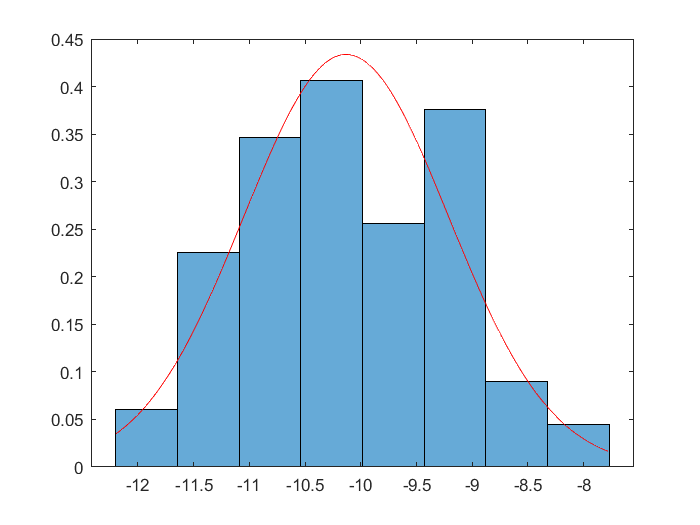
\includegraphics[scale=0.7]{imgs/hist_dens.png}
	\caption{Гистограмма и график функции плотности распределения вероятностей нормальной случайной величины с выборочным математическим ожиданием и исправленной выборочной  дисперсией}
	\label{fig:1}
\end{figure}

\begin{figure}[H]
	\centering
	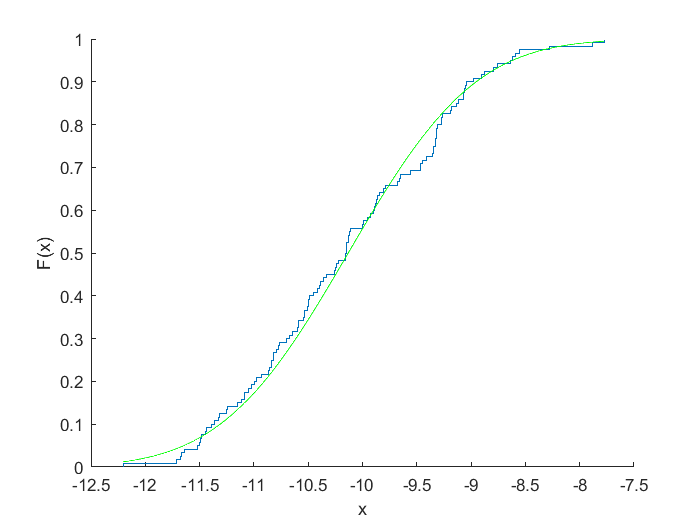
\includegraphics[scale=0.7]{imgs/func.png}
	\caption{График эмпирической функции распределения и функции распределения нормальной случайной величины с выборочным математическим ожиданием и исправленной выборочной  дисперсией}
	\label{fig:2}
\end{figure}

\end{document}